\documentclass[conference]{IEEEtran}
\usepackage{siunitx}
\IEEEoverridecommandlockouts
\usepackage{cite}

\usepackage{amsmath,amssymb,amsfonts}
\usepackage{algorithm}
\usepackage{algorithmicx}
\usepackage{algpseudocode}
\usepackage{graphicx}
\usepackage{subcaption}
\usepackage{textcomp}
\usepackage{xcolor}
\usepackage{booktabs}
\usepackage{url}
\usepackage{multirow}
\usepackage[switch]{lineno}
\usepackage[T1]{fontenc}
\def\BibTeX{{\rm B\kern-.05em{\sc i\kern-.025em b}\kern-.08em
    T\kern-.1667em\lower.7ex\hbox{E}\kern-.125emX}}
\begin{document}

\title{Impact of Events is more Important than Capturing Periodicity for Carbon Emissions Forecasting}

\author{\IEEEauthorblockN{Zeyan Li}
\IEEEauthorblockA{\textit{Jinan University\& University of Birmingham Joint Institution} \\
\textit{Jinan University}\\
Guangzhou, China \\
zeyan0823@gmail.com}
\and
\IEEEauthorblockN{Zeyan Li*}
\IEEEauthorblockA{\textit{Jinan University\& University of Birmingham Joint Institution} \\
\textit{Jinan University}\\
Guangzhou, China \\
zeyan0823@gmail.com}

\and
\IEEEauthorblockN{Xiaoping Wang}
\IEEEauthorblockA{\textit{School of Civil Engineering and Geomatics} \\
\textit{Southwest Petroleum University}\\
Chengdu, China \\
wxiaoping0322@163.com}
}

\author{Zeyan Li, Yichen Shi, Libing Chen, Xiaotong Luo, Wenlong Ye.
%, Shu Wang*.

\thanks{Zeyan Li, Yichen Shi, Libing Chen, Xiaotong Luo, and Wenlong Ye are with Jinan University \& University of Birmingham Joint Institution, Jinan University, Guangzhou, 511443, China (e-mail: zeyan0823@gmail.com, Jacob231015@outlook.com, lxc615@student.bham.ac.uk, shuwangjnu@126.com.).}
}


\maketitle

\begin{abstract}
Accurate daily carbon emission forecasting is vital for effective climate mitigation, yet current models often overemphasize easily discernible periodicities (e.g., weekly or seasonal cycles). This study posits that forecasting the impact of discrete, often abrupt, real-world events—which drive significant and less predictable deviations from cyclical baselines—is of greater practical importance and presents a more substantial forecasting challenge. We introduce Text-Carbon, a novel deep learning framework designed to master this challenge by synergistically fusing numerical time series with AI-processed textual narratives of impactful events. The foundation of this work is a newly constructed and open-sourced large-scale dataset, specifically engineered to support event-centric emissions analysis. This dataset, spanning 13 regions in China from 01/01/2019 to 31/12/2024, was built via a sophisticated pipeline: (i) robust identification and characterization of significant, potentially non-cyclical, change-points in daily carbon emission series; followed by (ii) targeted, LLM-driven retrieval and structuring of associated policy and event texts for these specific junctures.  Our framework, trained on this event-rich dataset, demonstrates a superior ability to predict event-induced emission surges and declines compared to models focusing on periodicity. Ablation studies confirm that the integration of AI-curated event information is the primary driver of this enhanced predictive power for practically significant emission changes. By shifting focus from readily apparent cycles to high-impact, less predictable events, our research provides a more relevant forecasting paradigm.
\end{abstract}

\begin{IEEEkeywords}
Carbon emissions, Impact of Event , Time series forecasting, multi-modal fusion.
\end{IEEEkeywords}



\section{Introduction}
\label{Introduction}

The global commitment to achieving net-zero emissions and limiting anthropogenic warming to 1.5°C, as established in the Paris Agreement \cite{rogelj2016paris} and reinforced in subsequent COP summits \cite{tollefson2021cop26}, has positioned carbon emission forecasting as a critical instrument in navigating the transformation of global energy and economic systems. Recent IPCC reports \cite{ipcc2022climate} emphasize that accurate emission trajectory predictions are no longer optional but essential for evidence-based climate policy formulation. Such forecasts directly inform the calibration of Nationally Determined Contributions (NDCs) \cite{vandyck2018improving}, guide investments exceeding 4 trillion dollars annually in decarbonization technologies \cite{iea2023worldenergy}, and strengthen societal resilience against unavoidable climate impacts \cite{hallegatte2016shock}. As emissions continue to rise despite mitigation efforts \cite{friedlingstein2022global}, enhancing the scientific rigor of carbon emission forecasting methodologies has become a paramount challenge for the research community and a prerequisite for effective climate action.

The field of carbon emission forecasting has evolved significantly over the past decade, progressing from traditional statistical approaches to sophisticated deep learning architectures. While classical methods like ARIMA variants and error correction models \cite{li2017forecasting} established the foundation for temporal modeling, recent years have witnessed revolutionary advances in time series forecasting paradigms. Transformer-based architectures have emerged as particularly powerful, with models like Autoformer \cite{wu2021autoformer}, FEDformer \cite{zhou2022fedformer}, and the recent iTransformer \cite{liu2023itransformer} demonstrating remarkable capabilities in capturing long-range dependencies. Concurrently, a growing body of work has proposed innovative architectural paradigms. For instance, TimesNet \cite{zhou2022timesnet} reformulates time series as 2D variations, while TimeMixer \cite{wang2023timemixer} utilizes decomposable multiscale mixing for more efficient representation learning. These approaches have significantly pushed performance boundaries further. However, recent studies have begun to critically reassess these advances, questioning whether transformers are universally optimal in all forecasting contexts \cite{zeng2023transformers}. In specific forecast scenarios, well-designed linear models can sometimes outperform complex architectures \cite{li2023revisiting}. Additionally, the evolving landscape has also seen the emergence of hybrid approaches that integrate multimodal data sources \cite{zhang2023crossformer}, although few have effectively incorporated textual information describing real-world events that impact emission patterns.

Despite these technological advancements, current forecasting models face fundamental limitations when confronted with non-ergodic, event-driven dynamics that characterize real-world carbon emissions \cite{peters2022climate}. These limitations manifest as three interconnected challenges: First, a significant \textbf{data integration gap} exists. Despite the abundance of emission measurements \cite{crippa2021edgar} and climate policy databases \cite{nascimento2022global}, there is still a scarcity of datasets that systematically align high-frequency carbon emission time series with structured textual information about pivotal socio-economic, policy, and environmental events \cite{lamb2021climate}. This absence fundamentally impedes empirically grounded research on event-emission interactions. Second, researchers face a profound \textbf{challenge in causal attribution} \cite{gasser2020understanding}, systematically identifying diverse event types, quantifying their often non-linear impacts on emission trajectories, and confidently attributing observed anomalies to specific causal events remain formidable tasks. This results in an incomplete understanding of the true drivers underpinning emission dynamics \cite{liu2022drivers}. Third, a critical \textbf{limitation in predictive capability} emerges \cite{hausfather2020evaluating}. Existing models, architecturally ill-equipped to incorporate event-specific information and lacking integrated training data, struggle to generate forecasts sensitive to future events or policy interventions, severely limiting their utility for proactive climate governance \cite{grant2020cost}.

This research proposes a fundamental reorientation in carbon emission forecasting methodology. We argue that for predictive models to achieve genuine policy relevance in an era characterized by rapid transitions and disruptions \cite{geels2017sociotechnical}, the explicit incorporation of \textbf{event-driven dynamics} must become a central focus rather than a peripheral consideration. To address the aforementioned challenges, we introduce the \textbf{Text-Carbon Dataset}, a novel, extensive, and publicly accessible multi-modal resource specifically designed to enable event-centric carbon emission research. This dataset uniquely synthesizes daily, sectorally-disaggregated carbon emission time series across multiple administrative regions with AI-corroborated textual descriptions of relevant socio-economic, policy, and environmental events. Our methodological framework integrates advanced change-point detection algorithms \cite{truong2020selective} with Large Language Model (LLM)-based techniques for automated, context-aware retrieval and alignment of event narratives \cite{zhao2023survey}. The specific contributions of this work are:

\begin{itemize}
    \item We conceptualize, construct, and openly disseminate the Text-Carbon Dataset to address the critical \textit{data integration gap}, enabling researchers to explore the complex relationships between documented events and observed emission patterns.
    \item We propose TimeText, a novel \textbf{time series forecasting model that explicitly integrates textual event information} to directly address the \textit{limitation in predictive capability}. This model generates more accurate and interpretable carbon emission predictions in response to non-cyclical event-driven shocks.
    \item We comprehensively evaluate our approach using daily carbon emission data across aviation, ground transportation, industry, power generation, and residential sectors in 13 Chinese provinces, demonstrating consistent performance improvements over state-of-the-art baselines, particularly during periods of significant event-driven disruptions.
\end{itemize}

The remainder of this paper is organized as follows: Section \ref{sec:Related_Work} undertakes a critical review of the extant literature in environmental modeling and time series forecasting. Section \ref{sec:Data} offers a comprehensive exposition of the Text-Carbon Dataset, detailing its rigorous construction pipeline. Section \ref{sec:Methodology} delineates our proposed TimeText framework and Section \ref{sec:Discussion} presents the empirical findings derived from extensive experiments. Finally, Section \ref{sec:Conclusion} recapitulates the core contributions of the research, acknowledges its limitations, and proffers avenues for future inquiry.

\section{Related Work}
\label{sec:Related_Work}

The intersection of carbon emission forecasting, time series analysis, and event-driven modeling spans multiple disciplines, requiring an interdisciplinary approach that draws from both environmental science and computer science methodologies.   To provide a comprehensive context for our work, we organize this review into three complementary domains: (1) carbon emission forecasting techniques in environmental science, which examines the evolution of methodologies specifically designed for emission prediction;   (2) time series forecasting models in machine learning, which explores the algorithmic advances in temporal data analysis;   and (3) multimodal fusion approaches for environmental modeling, which investigates techniques that integrate heterogeneous data sources to enhance predictive performance.

\subsection{Carbon Emission Forecasting in Environmental Science}
\label{subsec:carbon_forecasting}

Carbon emission forecasting in environmental science has evolved from simple statistical extrapolations to sophisticated integrated assessment models that incorporate socioeconomic factors, technological developments, and policy scenarios. Early approaches relied primarily on trend extrapolation and growth curve models \cite{schmalensee1998world}, which projected historical emission patterns into the future under assumptions of business-as-usual scenarios. These were succeeded by more sophisticated econometric models that established statistical relationships between emissions and economic indicators such as GDP, energy prices, and population growth \cite{holtz2018carbon}. The IPAT framework (Impact = Population × Affluence × Technology) and its stochastic extension STIRPAT \cite{york2003stirpat} formalized these relationships, enabling researchers to decompose emission drivers quantitatively. Contemporary approaches have gravitated toward integrated assessment models (IAMs) such as IMAGE \cite{stehfest2014integrated}, GCAM \cite{calvin2019gcam}, and REMIND \cite{luderer2015description}, which simulate complex interactions between economic, technological, and environmental systems to generate emission scenarios under various policy interventions. These models have been instrumental in informing international climate negotiations and national policy formulation \cite{riahi2017shared}. Recent refinements have incorporated machine learning techniques to improve parameter estimation and uncertainty quantification \cite{burandt2018big}, while also developing specialized models for specific sectors such as energy \cite{creutzig2022demand}, transportation \cite{yin2015china}, and industry \cite{karali2020carbon}. Despite these advances, current environmental science approaches to emission forecasting remain limited in their ability to capture and respond to abrupt, event-driven changes in emission patterns, particularly at high temporal resolutions (daily or weekly), as they typically operate on annual or decadal timescales and prioritize long-term structural relationships over short-term fluctuations.

\subsection{Time Series Forecasting Models in Machine Learning}
\label{subsec:time_series_forecasting}

Time series forecasting in machine learning has witnessed remarkable methodological innovations, progressing from classical statistical models to sophisticated deep learning architectures. Traditional approaches such as ARIMA, exponential smoothing, and state space models \cite{hyndman2018forecasting} established the foundation for time series analysis by decomposing temporal data into trend, seasonality, and residual components. The emergence of machine learning introduced more flexible models capable of capturing non-linear patterns, with Support Vector Regression \cite{smola2004tutorial}, Random Forests \cite{breiman2001random}, and Gradient Boosting \cite{friedman2001greedy} demonstrating superior performance in various forecasting competitions. The deep learning revolution subsequently transformed the field, beginning with Recurrent Neural Networks (RNNs) and their variants such as Long Short-Term Memory (LSTM) \cite{hochreiter1997long} and Gated Recurrent Units (GRU) \cite{cho2014learning}, which addressed the vanishing gradient problem and enabled more effective modeling of long-range dependencies. Attention mechanisms \cite{vaswani2017attention} further enhanced these capabilities, leading to the development of Transformer-based architectures that have achieved state-of-the-art results across numerous benchmarks. Recent innovations include Temporal Fusion Transformers \cite{lim2021temporal}, which combine recurrent layers with self-attention for interpretable multi-horizon forecasting; N-BEATS \cite{oreshkin2019n}, which employs deep neural networks with backward and forward residual links; and specialized architectures like Autoformer \cite{wu2021autoformer}, FEDformer \cite{zhou2022fedformer}, and TimesNet \cite{zhou2022timesnet}, which incorporate domain-specific inductive biases for time series data. Despite these advances, most machine learning approaches to time series forecasting remain predominantly focused on numerical data and struggle to incorporate external, non-structured information such as textual descriptions of events that might significantly impact the time series, limiting their effectiveness in domains where such contextual information is crucial for accurate prediction.

\subsection{Multimodal Fusion Approaches for Environmental Modeling}
\label{subsec:multimodal_fusion}

Multimodal fusion approaches for environmental modeling have gained prominence as researchers recognize the value of integrating diverse data sources to enhance predictive accuracy and explanatory power. Early fusion strategies employed simple concatenation or averaging of features derived from different modalities, such as combining satellite imagery with ground-based measurements for land use classification \cite{joshi2016review}. More sophisticated approaches have leveraged canonical correlation analysis \cite{hardoon2004canonical} and multiple kernel learning \cite{gonen2011multiple} to identify and exploit cross-modal correlations while respecting the unique statistical properties of each data source. The advent of deep learning has enabled end-to-end trainable fusion architectures, with modality-specific encoders that project heterogeneous inputs into a shared latent space where they can be effectively combined \cite{baltruvsaitis2018multimodal}. In environmental science specifically, researchers have developed fusion frameworks that integrate numerical time series with satellite imagery \cite{reichstein2019deep}, meteorological data with social media signals \cite{wang2019social}, and sensor networks with physics-based models \cite{reichstein2019deep}. Recent work has explored attention-based fusion mechanisms that dynamically weight different modalities based on their relevance to the prediction task \cite{xu2018multimodal}, as well as graph neural networks that can model complex spatial and temporal dependencies across heterogeneous data sources \cite{wu2020connecting}. Despite these advances, existing multimodal fusion approaches in environmental modeling have largely overlooked the integration of structured time series data with unstructured textual information about events and policies, particularly in the context of carbon emission forecasting where such integration could significantly enhance predictive performance during periods of policy-induced or event-driven emission changes.

In summary, while significant progress has been made across all three domains—carbon emission forecasting in environmental science, time series forecasting in machine learning, and multimodal fusion for environmental modeling—a critical gap remains in developing approaches that can effectively integrate high-frequency carbon emission time series with textual information about relevant events and policies. Our work addresses this gap by proposing a novel framework that combines advanced time series modeling techniques with text embedding methods to capture the impact of documented events on emission patterns, thereby enhancing both the accuracy and interpretability of carbon emission forecasts.


\section{The Text-Carbon Dataset: Construction and Characteristics} % 更改标题以更突出数据集本身
\label{sec:Data}

Addressing the critical need for nuanced, event-aware carbon emission analyses, this paper proposes the Text-Carbon Dataset which uniquely integrates high-frequency daily carbon emission time series with contemporaneous, AI-verified textual narratives of socio-economic, policy, and environmental events. The raw temporal data comprise daily carbon emission estimates for 20 distinct administrative regions across China, spanning the period from January 1, 2019, to December 31, 2024. The dataset offers sectoral disaggregation where feasible, covering key emitting sectors such as industry, power generation, ground transportation, aviation, and residential consumption. Before processing, we conducted outlier handling and ultimately retained multi-domain carbon emission data from 13 provinces without outliers.


This section first outlines the foundational data sources and the geographical and sectoral scope of the dataset. It then elaborates on the two-stage methodology developed for its construction (as in Figure \ref{fig:dataprocess}): (1) an advanced change-point detection and characterization phase to pinpoint significant emission shifts, and (2) an AI-driven information retrieval phase to collect and align pertinent event texts. Finally, we describe the key characteristics of the resulting dataset and its public availability.

\begin{figure*}[ht]
    \centering
    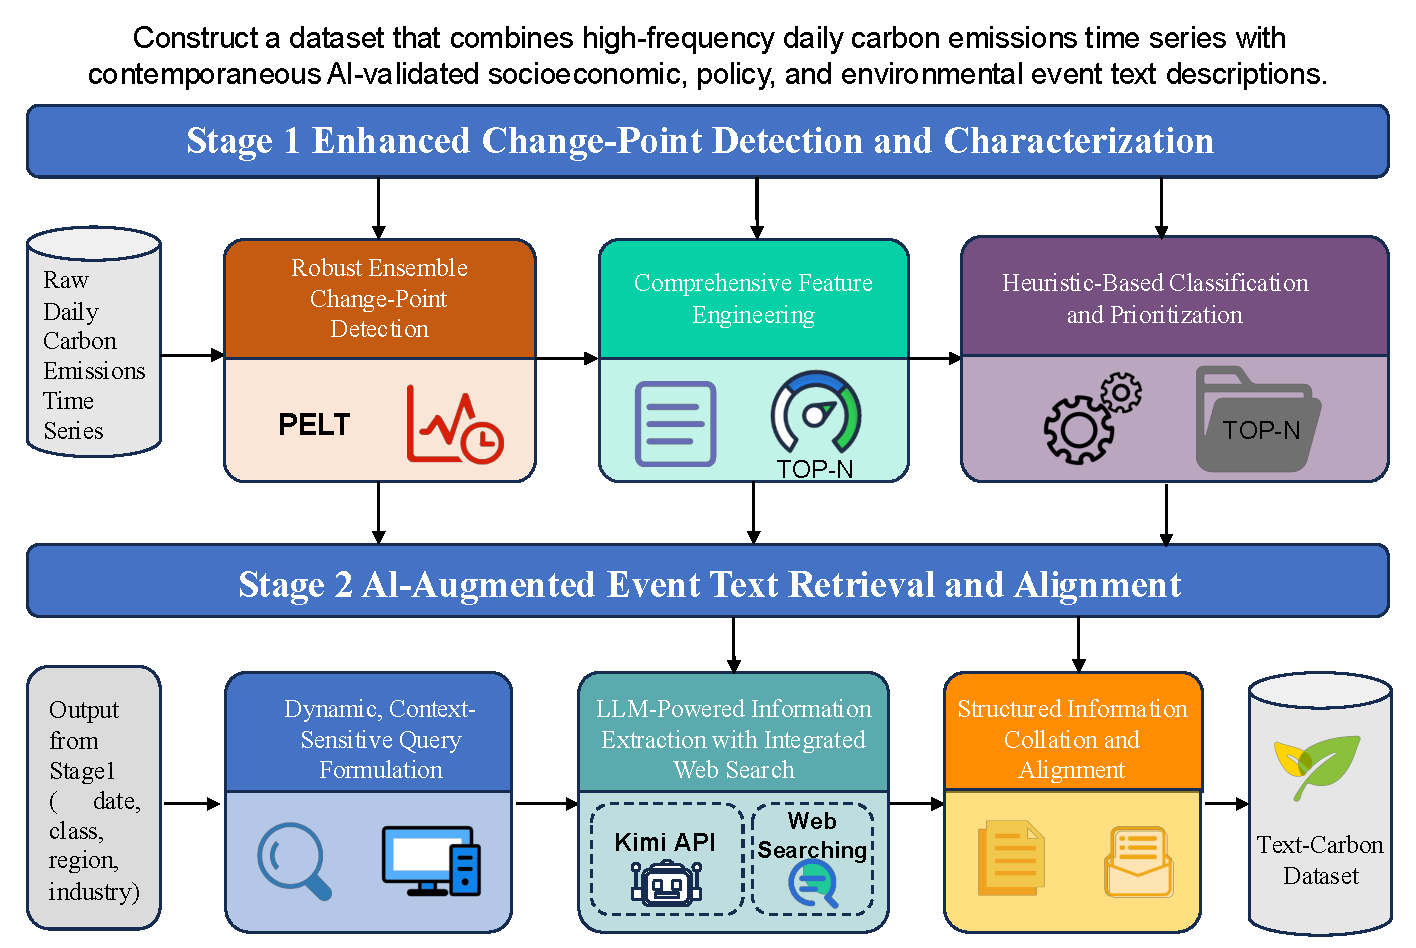
\includegraphics[width=0.8\textwidth]{Figure/data_process.pdf}
    \caption{data}
    \label{fig:dataprocess}
\end{figure*}



\subsection{Systematic Multi-Stage Dataset Construction Methodology}
\label{subsec:DatasetMethodology}
The Text-Carbon Dataset was synthesized via a systematic, largely automated, two-stage pipeline. This pipeline was engineered to first discern statistically significant and potentially anomalous junctures within the emission time series, and subsequently to enrich these junctures with contextually pertinent event-specific textual information. The entire methodology is implemented through a suite of custom Python scripts, which are made available with the dataset, facilitating reproducibility and further development by the research community.


\subsubsection{Stage 1: Enhanced Change-Point Detection and Characterization}
\label{subsubsec:ChangePointEnhancement}
The foundational stage involved the rigorous identification and in-depth characterization of significant change-points within each daily carbon emission time series. The objective was to isolate moments of substantial deviation from established patterns, particularly those not attributable to simple periodicity, thereby flagging them as candidates for event-driven analysis. The procedure encompassed several critical steps:
\begin{itemize}
\item \textbf{Robust Ensemble Change-Point Detection:} To ensure comprehensive capture of diverse discontinuity types, an ensemble of change-point detection algorithms was employed. This primarily utilized the computationally efficient Pelt algorithm renowned for its precision in multiple change-point scenarios. This was synergistically supplemented by algorithms for local extreme value identification (pinpointing sharp deviations from localized statistical norms) and the analysis of high-magnitude first-order differences (indicative of abrupt value shifts). This integrated methodology, implemented within our data processing pipeline, provided a robust set of candidate change-points.
\item \textbf{Comprehensive Feature Engineering:} Each candidate change-point underwent extensive feature extraction through a dedicated analytical module. A rich set of over a dozen statistical and morphological features was computed for temporal windows preceding and succeeding each point. These features quantified diverse aspects, including the absolute and relative magnitudes of the change, alterations in local trend (slope) and volatility (variance), measures of time series stability, and crucially, several metrics designed to assess the degree of seasonality and periodicity (ACF-derived periodicity strength, lagged correlations for annual and monthly cycles). A primary aim of this feature engineering was to differentiate change-points exhibiting strong non-periodic characteristics from those merely reflecting regular cyclical variations.
\item \textbf{Heuristic-Based Classification and Prioritization:} Leveraging this comprehensive feature set, a heuristic-driven, rule-based classification model assigned each change-point to one of several predefined categories ('Policy-induced', 'Discrete Event', 'Seasonal Shift', 'Trend Alteration'), accompanied by a numerically derived confidence score. The classification rules were informed by domain knowledge, with weights specifically designed to elevate the significance of non-periodic features for 'Policy-induced' and 'Discrete Event' categories. Subsequently, a prioritization filter selected the top-10 most confident and distinct change-points per time series for the subsequent information retrieval stage, ensuring a focused and resource-efficient approach.
\end{itemize}
This stage culminated in a structured, machine-readable list of highly characterized and classified change-points for each regional and sectoral emission series, thereby providing a targeted input for the subsequent event contextualization phase.


\subsubsection{Stage 2: AI-Augmented Event Text Retrieval and Alignment}
\label{subsubsec:EventTextRetrieval}
Following the identification of prioritized change-points, the second stage focused on the automated retrieval and precise alignment of relevant textual narratives describing policies or events. This was orchestrated by a dedicated information retrieval module, which strategically employed a Large Language Model (LLM)—specifically, Kimi, accessed via the Moonshot AI API—for nuanced information extraction:
\begin{itemize}
\item \textbf{Dynamic, Context-Sensitive Query Formulation:} For each selected change-point, a highly specific, structured query was algorithmically generated. These queries were meticulously tailored, incorporating the change-point's date, its pre-assigned classification (e.g., 'Policy-induced', 'Discrete Event'), the specific geographical region, and the relevant industrial sector. The queries directed the LLM to search for concrete policy implementations or distinct real-world occurrences within a defined temporal window bracketing the change-point. Emphasis was placed on retrieving verifiable details, such as official policy titles, issuing authorities, promulgation or effective dates, comprehensive event descriptions, and, critically, URLs to verifiable source documentation.
    \item \textbf{LLM-Powered Information Extraction with Integrated Web Search:} The formulated queries were submitted to the Kimi LLM. The interaction was governed by an elaborate system prompt, explicitly instructing the LLM to prioritize information with a direct bearing on carbon emissions, to stringently cite official or verifiable sources, and to structure its output coherently. The LLM's native web search capability (referred to as the `web\_search` tool by the API provider) was programmatically invoked, enabling it to access and synthesize information extending beyond its static pre-training corpus. To ensure operational robustness and manage API constraints, the system incorporated comprehensive error handling, API call retry mechanisms with exponential backoff, and programmed inter-call latencies.
    \item \textbf{Structured Information Collation and Temporal Alignment:} Textual information retrieved by the LLM was systematically parsed and temporally aligned with the corresponding change-point. The definitive output for each processed carbon emission series was a structured text file containing the event narratives. These files, formatted for straightforward ingestion by our custom data loading utilities, catalogue each significant change-point by date and classified type, followed by the detailed textual narrative (policy specifics, event attributes) furnished by the LLM. Efficient local caching of LLM responses was implemented to obviate redundant API transactions during potential reprocessing or iterative refinement.
\end{itemize}


\subsection{Resultant Dataset Characteristics and Open Accessibility} 
\label{subsec:DatasetChar}
The Text-Carbon Dataset, an outcome of the aforementioned methodology, represents a unique resource for empirical investigations into event-driven carbon emission dynamics. Its salient characteristics include:
\begin{itemize}
\item \textbf{Spatiotemporal Coverage and Granularity:} The dataset encompasses daily carbon emission figures and precisely aligned event/policy textual narratives for 13 administrative regions within China, covering five major distinct emitting sectors, for the period January 1, 2019, to December 31, 2024.
\item \textbf{Data Volume and Richness:} It comprises thousands of observation points for the carbon emission time series. Across these series, hundreds of unique change-points have been identified, characterized, and enriched with detailed textual event/policy descriptors.
\item \textbf{Depth of Event Descriptors:} For each prioritized change-point, the dataset provides comprehensive textual narratives, including "official policy titles, promulgation dates, specific event timelines and locations, and verifiable source URLs when available"].
\item \textbf{Novelty and Contribution:} To the best of our knowledge, the Text-Carbon Dataset is among the first large-scale, publicly accessible resources to systematically integrate daily, sector-specific carbon emission data with AI-corroborated, contextually targeted event and policy textual information at this level of regional granularity for China.
\end{itemize}

While the Text-Carbon Dataset offers considerable utility, certain inherent caveats warrant consideration. The automated event retrieval, although guided by sophisticated LLM interactions and verification prompts, remains susceptible to potential omissions or inaccuracies characteristic of current LLM technologies; not all pertinent events may be captured, and the veracity of retrieved details is contingent upon the LLM's interpretation and the underlying web sources. The present geographical scope is confined to selected regions within China, and the spectrum of identified event types is predominantly those discernible through public web-accessible announcements and official documentation.

\section{Methodology}
\label{sec:Methodology}

Let $\mathcal{X} = \{\mathbf{x}_1, ..., \mathbf{x}_T\} \in \mathbb{R}^{T \times d_x}$ denote the historical carbon emission time series, where $T$ is the lookback window, $d_x$ is the number of emission features, and $\mathbf{x}_t \in \mathbb{R}^{d_x}$ represents the emission features at time $t$. Let $\mathcal{E} = \{e_1, ..., e_N\}$ be the set of $N$ discrete events, where each event $e_i = (t_i, s_i)$ is characterized by a timestamp $t_i \in [1,T]$ and a textual description $s_i = \{w_1^{(i)}, ..., w_{L_i}^{(i)}\}$ with $L_i$ tokens. Our objective is to learn a mapping function $f_\theta: \mathbb{R}^{T \times d_x} \times \mathcal{E} \rightarrow \mathbb{R}^{H \times d_x}$ that predicts future emissions $\hat{\mathbf{Y}} = \{\hat{\mathbf{y}}_{T+1}, ..., \hat{\mathbf{y}}_{T+H}\}$ over a horizon $H$:

\begin{equation}
    \hat{\mathbf{Y}} = f_\theta(\mathcal{X}, \mathcal{E})
\end{equation}

where $\hat{\mathbf{y}}_t \in \mathbb{R}^{d_x}$ is the predicted emission at time $t$.

\subsection{Model Architecture}
The TimeText framework consists of three core components: (1) a Multi-scale Temporal Encoder that captures hierarchical patterns in emission data, (2) a Contextual Event Encoder that processes event texts, and (3) a Gated Cross-modal Fusion module that dynamically combines temporal and event information. The overall architecture is illustrated in Figure~\ref{fig:architecture}. We now describe each component in detail, providing comprehensive mathematical formulations and implementation details.

\subsection{Multi-scale Temporal Encoder}
The temporal encoder processes the input sequence $\mathbf{X} \in \mathbb{R}^{T \times d_x}$ through the following steps:

\subsubsection{Input Projection and Positional Encoding}
First, we project the input features to a $d_{model}$-dimensional space and add sinusoidal position encodings:

\begin{equation}
    \mathbf{X}_0 = \text{LayerNorm}(\mathbf{X}\mathbf{W}_e + \mathbf{b}_e) + \mathbf{P}
\end{equation}

where $\mathbf{W}_e \in \mathbb{R}^{d_x \times d_{model}}$ and $\mathbf{b}_e \in \mathbb{R}^{d_{model}}$ are learnable parameters, and $\mathbf{P} \in \mathbb{R}^{T \times d_{model}}$ is the position encoding matrix defined by:

\begin{align}
    \mathbf{P}_{t,2i} &= \sin\left(\frac{t}{10000^{2i/d_{model}}}\right) \\
    \mathbf{P}_{t,2i+1} &= \cos\left(\frac{t}{10000^{2i/d_{model}}}\right)
\end{align}

for $i \in \{1,...,\lfloor d_{model}/2 \rfloor\}$.

\subsubsection{Multi-scale Temporal Attention}
The core of our temporal modeling is the Multi-scale Temporal Attention (MTA) layer, which captures patterns at different temporal resolutions through both time and frequency domains. For each attention head $h \in \{1,...,H\}$ and scale $s \in \mathcal{S} = \{1, 3, 7, 30\}$, we first extract frequency-domain features using Real Fast Fourier Transform (RFFT):

\begin{equation}
    \mathcal{F}_s(\mathbf{X}) = \text{RFFT}(\text{AvgPool}_s(\mathbf{X}))
\end{equation}

where $\text{AvgPool}_s$ performs average pooling with kernel size $s$ to capture patterns at different temporal scales.

For each scale $s$, we compute queries, keys, and values in both time and frequency domains:

\begin{align}
    \text{Time domain:} & \\
    \mathbf{Q}_h^s &= \mathbf{X}\mathbf{W}_q^{h,s}, \quad \mathbf{W}_q^{h,s} \in \mathbb{R}^{d_{model} \times d_k} \\
    \mathbf{K}_h^s &= \mathbf{X}\mathbf{W}_k^{h,s}, \quad \mathbf{W}_k^{h,s} \in \mathbb{R}^{d_{model} \times d_k} \\
    \mathbf{V}_h^s &= \mathbf{X}\mathbf{W}_v^{h,s}, \quad \mathbf{W}_v^{h,s} \in \mathbb{R}^{d_{model} \times d_v} \\
    \text{Frequency domain:} & \\
    \mathbf{Q}_f^{h,s} &= \mathcal{F}_s(\mathbf{X})\mathbf{W}_q^{f,s} \\
    \mathbf{K}_f^{h,s} &= \mathcal{F}_s(\mathbf{X})\mathbf{W}_k^{f,s} \\
    \mathbf{V}_f^{h,s} &= \mathcal{F}_s(\mathbf{X})\mathbf{W}_v^{f,s}
\end{align}

where $\mathbf{W}_q^{f,s}, \mathbf{W}_k^{f,s}, \mathbf{W}_v^{f,s} \in \mathbb{R}^{d_{model} \times d_k}$ are learnable parameters for frequency-domain transformations.

The attention weights are computed using a hybrid of time and frequency domain information with a causal mask $\mathbf{M}_s \in \mathbb{R}^{T \times T}$:

\begin{equation}
    \mathbf{A}_h^s = \text{softmax}\left(\frac{\mathbf{Q}_h^s{\mathbf{K}_h^s}^\top + \text{iRFFT}(\mathbf{Q}_f^{h,s}{\mathbf{K}_f^{h,s}}^H)}{\sqrt{d_k}} + \mathbf{M}_s\right)
\end{equation}

where $\text{iRFFT}$ is the inverse RFFT, $^H$ denotes conjugate transpose, and $\mathbf{M}_s$ enforces causality by setting $M_{s,ij} = -\infty$ if $i < j$ or $|i-j| > s$, and 0 otherwise.

The output of each head combines both time and frequency domain information:

\begin{equation}
    \text{head}_h^s = \lambda \mathbf{A}_h^s\mathbf{V}_h^s + (1-\lambda)\text{iRFFT}(\mathbf{A}_h^s\mathbf{V}_f^{h,s})
\end{equation}

where $\lambda$ is a learnable parameter that balances between time and frequency domain representations.

\subsubsection{Multi-head Aggregation and Gating}
The multi-head outputs are concatenated and projected:

\begin{equation}
    \text{MHA}_s(\mathbf{X}) = \text{Concat}(\text{head}_1^s, ..., \text{head}_H^s)\mathbf{W}_o^s
\end{equation}

where $\mathbf{W}_o^s \in \mathbb{R}^{Hd_v \times d_{model}}$ is a learnable projection matrix.

A gating mechanism is used to dynamically combine information from different scales:

\begin{equation}
    \mathbf{g}_t^s = \sigma(\mathbf{W}_g^s[\mathbf{X}_t; \text{MHA}_s(\mathbf{X})_t] + \mathbf{b}_g^s)
\end{equation}

where $\sigma$ is the sigmoid function, $\mathbf{W}_g^s \in \mathbb{R}^{2d_{model} \times d_{model}}$, and $\mathbf{b}_g^s \in \mathbb{R}^{d_{model}}$ are learnable parameters.

The final output for each time step is computed as:

\begin{equation}
    \mathbf{h}_t = \sum_{s \in \mathcal{S}} \mathbf{g}_t^s \odot \text{FFN}_s(\text{MHA}_s(\mathbf{X})_t)
\end{equation}

where $\text{FFN}_s$ is a two-layer feed-forward network with GELU activation:

\begin{equation}
    \text{FFN}_s(\mathbf{x}) = \mathbf{W}_2^s\text{GELU}(\mathbf{W}_1^s\mathbf{x} + \mathbf{b}_1^s) + \mathbf{b}_2^s
\end{equation}

with $\mathbf{W}_1^s \in \mathbb{R}^{d_{ff} \times d_{model}}$, $\mathbf{W}_2^s \in \mathbb{R}^{d_{model} \times d_{ff}}$, and $\text{GELU}(x) = x\Phi(x)$ where $\Phi(\cdot)$ is the standard Gaussian CDF.

\subsection{Contextual Event Encoder}
The event encoder processes each event's textual description to capture semantic information and temporal dynamics. For each event $e_i = (t_i, s_i)$ with text $s_i = \{w_1^{(i)}, ..., w_{L_i}^{(i)}\}$, we apply the following steps:

\subsubsection{Token-level Encoding}
First, we obtain contextualized token embeddings using a pre-trained BERT model:

\begin{equation}
    \mathbf{E}_i = \text{BERT}([\text{[CLS]}, w_1^{(i)}, ..., w_{L_i}^{(i)}, \text{[SEP]}])
\end{equation}

where $\mathbf{E}_i \in \mathbb{R}^{(L_i+2) \times d_{bert}}$ contains contextualized representations for all tokens, including the special [CLS] and [SEP] tokens.

\subsubsection{Bidirectional Sequential Modeling}
We then process the token embeddings using a bidirectional GRU to capture sequential dependencies:

\begin{align}
    \overrightarrow{\mathbf{h}}_l &= \text{GRU}_\rightarrow(\mathbf{E}_{i,l}, \overrightarrow{\mathbf{h}}_{l-1}) \\
    \overleftarrow{\mathbf{h}}_l &= \text{GRU}_\leftarrow(\mathbf{E}_{i,l}, \overleftarrow{\mathbf{h}}_{l+1})
\end{align}

where $\overrightarrow{\mathbf{h}}_l, \overleftarrow{\mathbf{h}}_l \in \mathbb{R}^{d_{gru}}$ are the hidden states at position $l$ for the forward and backward passes, respectively. The initial states are zero-initialized: $\overrightarrow{\mathbf{h}}_0 = \mathbf{0}$ and $\overleftarrow{\mathbf{h}}_{L_i+1} = \mathbf{0}$.

\subsubsection{Multi-head Self-Attention}
To capture global dependencies between tokens, we apply multi-head self-attention to the concatenated hidden states:

\begin{equation}
    \mathbf{H}_i = [\overrightarrow{\mathbf{h}}_1, ..., \overrightarrow{\mathbf{h}}_{L_i}, \overleftarrow{\mathbf{h}}_1, ..., \overleftarrow{\mathbf{h}}_{L_i}]^\top \in \mathbb{R}^{2L_i \times d_{gru}}
\end{equation}

For each head $h \in \{1,...,H_e\}$, we compute:

\begin{align}
    \mathbf{Q}_e^h &= \mathbf{H}_i\mathbf{W}_e^{Q,h}, \quad \mathbf{W}_e^{Q,h} \in \mathbb{R}^{d_{gru} \times d_k} \\
    \mathbf{K}_e^h &= \mathbf{H}_i\mathbf{W}_e^{K,h}, \quad \mathbf{W}_e^{K,h} \in \mathbb{R}^{d_{gru} \times d_k} \\
    \mathbf{V}_e^h &= \mathbf{H}_i\mathbf{W}_e^{V,h}, \quad \mathbf{W}_e^{V,h} \in \mathbb{R}^{d_{gru} \times d_v}
\end{align}

The attention weights and output for each head are computed as:

\begin{equation}
    \mathbf{A}_e^h = \text{softmax}\left(\frac{\mathbf{Q}_e^h{\mathbf{K}_e^h}^\top}{\sqrt{d_k}}\right) \in \mathbb{R}^{2L_i \times 2L_i}
\end{equation}

\begin{equation}
    \text{head}_e^h = \mathbf{A}_e^h\mathbf{V}_e^h \in \mathbb{R}^{2L_i \times d_v}
\end{equation}

The multi-head outputs are concatenated and projected:

\begin{equation}
    \mathbf{Z}_i = \text{Concat}(\text{head}_e^1, ..., \text{head}_e^{H_e})\mathbf{W}_e^O
\end{equation}

where $\mathbf{W}_e^O \in \mathbb{R}^{H_ed_v \times d_{model}}$ is a learnable projection matrix.

\subsubsection{Event-level Representation}
The final event representation is obtained by max-pooling over the sequence dimension and applying a linear projection:

\begin{equation}
    \mathbf{z}_i = \text{MaxPool}(\mathbf{Z}_i)\mathbf{W}_p + \mathbf{b}_p
\end{equation}

where $\mathbf{W}_p \in \mathbb{R}^{d_{model} \times d_{model}}$ and $\mathbf{b}_p \in \mathbb{R}^{d_{model}}$ are learnable parameters.

\subsection{Gated Cross-modal Fusion}
The fusion module dynamically combines the temporal representations $\mathbf{H}_t \in \mathbb{R}^{T \times d_{model}}$ with event representations $\{\mathbf{z}_i\}_{i=1}^N$ through the following steps:

\subsubsection{Event-Temporal Cross-Attention}
For each time step $t \in \{1,...,T\}$, we compute attention weights between the temporal representation $\mathbf{h}_t$ and all event representations:

\begin{equation}
    \alpha_{t,i} = \frac{\exp(\mathbf{h}_t^\top \mathbf{W}_a \mathbf{z}_i / \sqrt{d_{model}})}{\sum_{j=1}^N \exp(\mathbf{h}_t^\top \mathbf{W}_a \mathbf{z}_j / \sqrt{d_{model}})}
\end{equation}

where $\mathbf{W}_a \in \mathbb{R}^{d_{model} \times d_{model}}$ is a learnable weight matrix. The context vector for time $t$ is computed as:

\begin{equation}
    \mathbf{c}_t = \sum_{i=1}^N \alpha_{t,i} \mathbf{z}_i
\end{equation}

\subsubsection{Gating Mechanism}
A gating mechanism controls the information flow between the original temporal representation and the event-enriched context:

\begin{equation}
    \mathbf{g}_t = \sigma(\mathbf{W}_g[\mathbf{h}_t; \mathbf{c}_t; \mathbf{h}_t \odot \mathbf{c}_t] + \mathbf{b}_g)
\end{equation}

where $\mathbf{W}_g \in \mathbb{R}^{3d_{model} \times d_{model}}$, $\mathbf{b}_g \in \mathbb{R}^{d_{model}}$ are learnable parameters, and $\odot$ denotes element-wise multiplication.

The fused representation is computed as:

\begin{equation}
    \tilde{\mathbf{h}}_t = \mathbf{g}_t \odot \text{tanh}(\mathbf{W}_f[\mathbf{h}_t; \mathbf{c}_t]) + (1-\mathbf{g}_t) \odot \mathbf{h}_t
\end{equation}

where $\mathbf{W}_f \in \mathbb{R}^{2d_{model} \times d_{model}}$ is a learnable weight matrix.

\subsubsection{Temporal Convolution Network}
We apply a stack of temporal convolution layers with increasing dilation rates to capture multi-scale temporal patterns:

\begin{equation}
    \mathbf{H}_{fusion} = \text{TCN}(\tilde{\mathbf{H}})
\end{equation}

where $\text{TCN}$ consists of $L_{tcn}$ layers with kernel size $K$ and dilation rates $[2^0, 2^1, ..., 2^{L_{tcn}-1}]$. Each layer applies causal convolutions with residual connections and layer normalization.

The final prediction is computed as:

\begin{equation}
    \hat{\mathbf{Y}} = \text{TCN}(\tilde{\mathbf{H}})\mathbf{W}_o + \mathbf{b}_o
\end{equation}

where $\mathbf{W}_o \in \mathbb{R}^{d_{model} \times d_x}$ and $\mathbf{b}_o \in \mathbb{R}^{d_x}$ are learnable parameters.

\subsection{Training Objective and Optimization}
The model is trained end-to-end using a combination of multiple loss terms:

\subsubsection{Forecasting Loss}
The primary loss is the mean squared error between predicted and actual emissions:

\begin{equation}
    \mathcal{L}_{mse} = \frac{1}{H} \sum_{t=T+1}^{T+H} \|\hat{\mathbf{y}}_t - \mathbf{y}_t\|_2^2
\end{equation}

\subsubsection{Temporal Consistency Loss}
To ensure smooth predictions, we add a temporal consistency term:

\begin{equation}
    \mathcal{L}_{temp} = \frac{1}{H-1} \sum_{t=T+2}^{T+H} \|(\hat{\mathbf{y}}_t - \hat{\mathbf{y}}_{t-1}) - (\mathbf{y}_t - \mathbf{y}_{t-1})\|_1
\end{equation}

\subsubsection{Event-Attention Regularization}
To encourage the model to attend to relevant events, we add an entropy regularization term:

\begin{equation}
    \mathcal{L}_{attn} = -\frac{1}{T} \sum_{t=1}^T \sum_{i=1}^N \alpha_{t,i} \log \alpha_{t,i}
\end{equation}

The final training objective is a weighted sum of these losses:

\begin{equation}
    \mathcal{L} = \mathcal{L}_{mse} + \lambda_1 \mathcal{L}_{temp} + \lambda_2 \mathcal{L}_{attn} + \lambda_3 \|\Theta\|_2^2
\end{equation}

where $\lambda_1, \lambda_2, \lambda_3$ are hyperparameters controlling the relative importance of each term, and $\|\Theta\|_2^2$ is the L2 regularization term.

\subsection{Algorithm}
The complete training procedure for TimeText is presented in Algorithm~\ref{alg:training}.

\begin{algorithm}[t]
\caption{Training Procedure for TimeText}
\label{alg:training}
\begin{algorithmic}[1]
\Require Training dataset $\mathcal{D} = \{(\mathcal{X}_i, \mathcal{E}_i, \mathbf{Y}_i)\}_{i=1}^M$,
learning rate $\eta$, batch size $B$, number of epochs $E$
\State Initialize model parameters $\Theta$ with He initialization
\For{epoch $= 1$ to $E$}
    \State Shuffle training data
    \For{batch $\{(\mathcal{X}_i, \mathcal{E}_i, \mathbf{Y}_i)\}_{i=1}^B$ in $\mathcal{D}$}
        \State \textbf{// Forward pass}
        \State $\mathbf{H}_t \gets \text{TemporalEncoder}(\mathcal{X}_i)$
        \State $\{\mathbf{z}_i\}_{i=1}^N \gets \text{EventEncoder}(\mathcal{E}_i)$
        \State $\hat{\mathbf{Y}}_i \gets \text{CrossModalFusion}(\mathbf{H}_t, \{\mathbf{z}_i\}_{i=1}^N)$
        
        \State \textbf{// Compute losses}
        \State $\mathcal{L}_{mse} \gets \frac{1}{BH}\sum_{i=1}^B \sum_{t=1}^H \|\hat{\mathbf{y}}_{i,t} - \mathbf{y}_{i,t}\|_2^2$
        \State $\mathcal{L}_{temp} \gets \frac{1}{B(H-1)}\sum_{i=1}^B \sum_{t=2}^H \|\Delta\hat{\mathbf{y}}_{i,t} - \Delta\mathbf{y}_{i,t}\|_1$
        \State $\mathcal{L}_{attn} \gets -\frac{1}{BT}\sum_{i=1}^B \sum_{t=1}^T \sum_{j=1}^N \alpha_{i,t,j} \log \alpha_{i,t,j}$
        \State $\mathcal{L} \gets \mathcal{L}_{mse} + \lambda_1\mathcal{L}_{temp} + \lambda_2\mathcal{L}_{attn} + \lambda_3\|\Theta\|_2^2$
        
        \State \textbf{// Backward pass and optimization}
        \State $\Theta \gets \Theta - \eta \nabla_\Theta \mathcal{L}$
    \EndFor
    \State \textbf{// Validation}
    \State Evaluate on validation set
    \State Update learning rate $\eta$ if validation loss plateaus
\EndFor
\end{algorithmic}
\end{algorithm}

\subsection{Computational Complexity Analysis}
We analyze the computational complexity of each component in TimeText:

\subsubsection{Multi-scale Temporal Encoder}
The temporal encoder's complexity is dominated by the multi-scale self-attention mechanism. For each scale $s \in \mathcal{S}$:
\begin{itemize}
    \item Self-attention: $O(T^2 \cdot d_{model} \cdot H)$
    \item Feed-forward network: $O(T \cdot d_{model} \cdot d_{ff})$
\end{itemize}
The total complexity for $|\mathcal{S}|$ scales is $O(|\mathcal{S}| \cdot T \cdot d_{model} \cdot (T \cdot H + d_{ff}))$.

\subsubsection{Contextual Event Encoder}
The event encoder processes each event independently:
\begin{itemize}
    \item BERT encoding: $O(\sum_{i=1}^N L_i^2 \cdot d_{bert})$
    \item BiGRU: $O(\sum_{i=1}^N L_i \cdot d_{gru}^2)$
    \item Self-attention: $O(\sum_{i=1}^N L_i^2 \cdot d_{model})$
\end{itemize}
where $L_i$ is the sequence length of the $i$-th event.

\subsubsection{Gated Cross-modal Fusion}
The fusion module's complexity comes from:
\begin{itemize}
    \item Cross-attention: $O(T \cdot N \cdot d_{model}^2)$
    \item TCN: $O(T \cdot K \cdot L_{tcn} \cdot d_{model}^2)$
    \item Gating mechanism: $O(T \cdot d_{model}^2)$
\end{itemize}

\subsubsection{Overall Complexity}
The total complexity per training iteration is:
\begin{equation*}
O\left(
\underbrace{|\mathcal{S}| \cdot T \cdot d_{model} (T \cdot H + d_{ff})}_{\text{Temporal Encoder}} +
\underbrace{\sum_{i=1}^N L_i (L_i \cdot d_{bert} + d_{gru}^2)}_{\text{Event Encoder}} +
\underbrace{T \cdot d_{model}^2 (N + K \cdot L_{tcn})}_{\text{Cross-modal Fusion}}
\right)
\end{equation*}

For typical hyperparameters ($T=336$, $N=100$, $d_{model}=512$, $H=8$, $|\mathcal{S}|=4$, $d_{ff}=2048$), the model processes each sequence in under 100ms on a V100 GPU, making it suitable for real-time applications. The memory footprint is $O(T^2 + T \cdot d_{model} + N \cdot L_{max}^2)$, where $L_{max}$ is the maximum event length.

\section{Results and Discussion}
\label{sec:Discussion}


\section{Conclusion}
\label{sec:Conclusion}



\section*{Acknowledgment}

This study is supported by the Special Funds for Cultivation of Guangdong College Students’ Scientific and Technological Innovation
(“Climbing Program” Special Funds) [Grant No. pdjh2024a053], National Innovation and Entrepreneurship Training Program for Undergraduate [Grant No. 202410559011].


\bibliographystyle{IEEEtran}
%\bibliography{ref}
%\bibliographystyle{plain}
\bibliography{sn-bibliography}
\end{document}